\chapter{Conclusie}
\label{cha:conclusie}
Het doel van dit rapport was het ontwerpen van een 'Pakkethondje' dat een gewicht van 10 kg over een hindernisbaan kan transporteren. De belangrijkste criteria bij dit ontwerp was het kunnen overnemen van een obstakel. 

Tijdens het ontwerpproces zijn vier kansrijke ontwerpen ontwikkeld: de 'Mantis Car', de 'Uitschuiver', de 'inklapper' en de 'Vierpoter'. Van deze ontwerpen zijn prototypes gemaakt die werden getest op de prestatiecriteria. Uit de testen bleek dat het meest kansrijke ontwerp een samenstelling is van de vier prototypes. Er is gekozen voor het mechanisme van de driepoot waarbij de schaarliften van de uitschuiver worden gebruikt. Dit eindontwerp gaat onder de naam 'Driepoter'.
%zie figuur blabla

De voornaamste reden voor het kiezen van de schaarlift is dat het stabieler is dan de andere deelontwerpen. Het schaarliftmechanisme presteerde beter omtrent stabiliteit dan de grijphaken en de inklapbare poten. Een tweede reden voor het kiezen van de schaarlift is in verband met de lengte van het voertuig. Het gebruik van inklapbare poten vereist een zeer lange kar, wat zorgt voor problemen tijdens het sturen. Met het gebruik van schaarliften kan het voertuig korter worden. Een andere reden voor de schaarlift is de veelzijdigheid van het ontwerp. Schaarliften kunnen gemakkelijk een verticale beweging opdoen, waardoor het over de meeste obstakels kan rijden. Grijphaken van de Mantis Car kunnen maximaal obstakels van maximaal 20 cm nemen terwijl de schaarlift tweemaal die hoogte kan leveren.

Hoewel de schaarlift de beste keuze blijkt te zijn, zijn er nog onzekerheden wat betreft trillingen op het systeem. Er is op gerekend dat alle staven alleen worden belast op druk, hoewel de aanwezigheid van trillingen kan zorgen voor ongewenste extra krachten op de staven. Er zullen experimenten moeten worden gedaan om een duidelijker beeld te krijgen op de invloed van trillingen op het systeem. 

\begin{figure}[H]
    \centering
    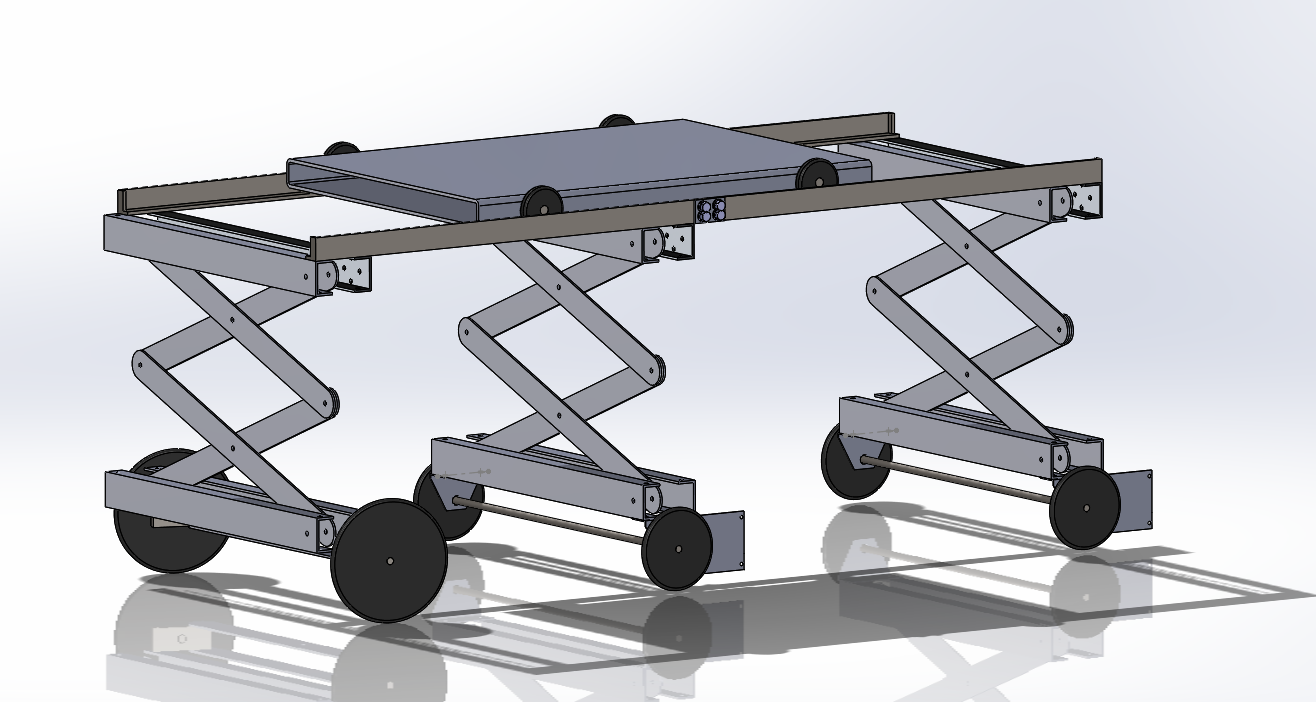
\includegraphics[width = 100mm]{05_conclusie/eindconcept.jpg}
    \caption{Solidworksmodel van het eindconcept}
    \label{eindconcept}
\end{figure}
